%      % SOCKETS
\subsection{Network programming --- sockets}%
\label{sec:netw-progr-sock}
Computer systems implement multiple processes which require an identifier. As
such, the IP address is not enough to uniquely identify the origin/destination
of data to be transmitted, and the port number is added. This combination of an
IP address and port number is sometimes called a network socket~\cite{wright1995tcp}, allowing
data to be delivered to multiple processes in the same machine --- same IP
address.
It is the socket pair (the 4-tuple consisting of the client IP address, client
port number, server IP address, and server port number) that specifies the two
end points that uniquely identifies each TCP connection in an
internet~\cite{wright1995tcp}. Bluetooth, as aforementioned, also uses sockets
for multiprocess communication, given the device address, transport protocol and
port number~\cite{huang2007bluetooth}.

In a broader sense, a socket can be described as a method of \gls{ipc} that allows data to be exchanged between applications, either on
the same host (computer) or on different hosts connected by a network~\cite{kerrisk2010linux}, as a
local interface to a system, created by the applications and controlled by the
operating system, allowing an application process to simultaneously send and
receive messages from other processes.

The Socket API was created in UNIX BSD 4.1 in 1981, with widespread
implementation in UNIX BSD 4.2~\cite{kerrisk2010linux}. It implements the Client-Server paradigm and
implement several (standard) functions to access the operating system network
resources, through system calls, in Linux~\cite{kerrisk2010linux}.

There are two generic ways to use sockets: for outgoing connections --- client
socket --- and for incoming connections --- server
socket. Fig.~\ref{fig:sockets-connection} illustrates the required steps to
obtain a connected socket:
\begin{enumerate}
\item When a socket is initially created is mostly unuseful.
\item Binding the server socket associates it to an unique network tuple (address and
  port number), enabling it to be uniquely addressed.
\item When a socket server goes into listening mode, the remote devices can
  initiate the connection procedure, referring to its unique network tuple.
\item When the socket server accepts a connection, it spawns a new socket which
  is connected to the remote device, and the endpoints can effectively
  communicate. The server socket is ready to accept new incomming connections.
\end{enumerate}
\newpage
% Sockets connection
\begin{figure}[!hbt]
\centering
    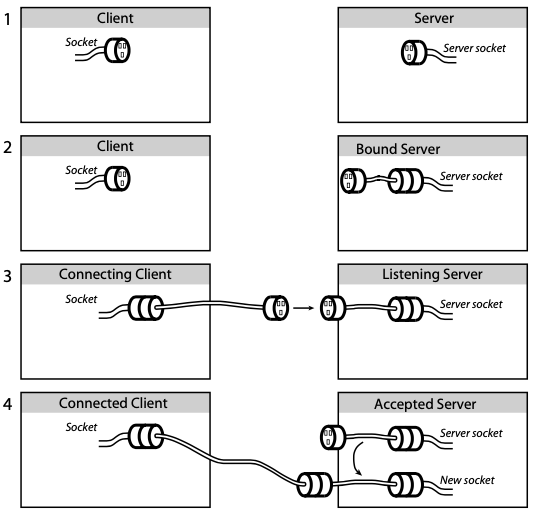
\includegraphics[width=0.4\textwidth]{./img/sockets-connection.png}
  \caption{Steps to obtain a connected socket (withdrawn from~\cite{huang2007bluetooth})}%
\label{fig:sockets-connection}
\end{figure}
%
%%% Local Variables:
%%% mode: latex
%%% TeX-master: "../../../dissertation"
%%% End:
